
\chapter{Универсальность полученных результатов}

Анализ модельного порыва позволил выделить основные элементы механизма поддержания колебаний в этом решении. В настоящей главе поднимается вопрос об универсальности полученных результатов. В главе приведены результаты исследования механизма поддержания колебаний в нескольких инвариантных решениях уравнений Навье-Стокса, отличных от модельного порыва. Инвариантными мы называем решения, которые не меняются при переходе к новой системе отчета, отличающейся от исходной сдвигом во времени или в пространстве. В настоящее время известно достаточно большое число различных инвариантных решений уравнений Навье-Стокса \cite{Kawahara2012}. Наиболее простым примером трехмерных инварианты решений являются бегущие волны. Их поле скорости периодично вдоль потока и стационарно в подходящей подвижной системе отсчета. Более сложным примером являются условно периодические решения, то есть решения, являющиеся периодическими по времени в подходящей подвижной системе отсчета. Частным случаем условно периодического решения является модельный порыв. Пользуясь простотой временного поведения таких решений, мы можем выполнить их детальное исследование. 


В главе дано описание метода Ньютона-Крылова, позволяющего находить условно периодические решения уравнений Навье-Стокса. Как частный случай условно периодических решений, метод позволяет находить решения, имеющие вид бегущей волны. Также в главе дано описание метода продолжения по параметру, опирающегося на метод Ньютона-Крылова. Опираясь на модельный порыв методом продолжения по параметру в работе найдено семейство условно периодических решений уравнений Навье-Стокса с пространственно локализованной структурой. В соответствии с \cite{Avila2013}, среди найденных таким образом решений существуют решения, по ряду качественных характеристик оказывающиеся ближе к турбулентному порыву, чем модельный порыв.  Также в работе было найдено несколько семейств решений уравнений Навье-Стокса, имеющих вид бегущей волны, описывающих движение жидкости в круглой трубе и в плоском канале. Описаны основные характеристик найденных решений и механизм поддержания колебаний в них. Во всех исследованных решениях основные элементы механизма поддержания колебаний оказываются такими же, как и в модельном порыве, что в некоторой степени говорит об универсальности этого механизма. Анализ решений в виде бегущей волны, описывающих движение жидкости в плоском канале, опубликован в работах автора \cite{Vest18, KMU2016}. 


\section{Метод Ньютона-Крылова для поиска условно периодических решений уравнений Навье-Стокса} \label{Newton_seq}

Условно периодическим мы называем решение уравнений Навье-Стокса, являющееся периодическим по времени в подходящей подвижной системе отсчета. В работе реализован метод Ньютона-Крылова \cite{Sanchez2004, Viswanath2007, Dijkstra2014}, позволяющий численно находить мгновенные поля скорости, соответствующие условно периодическим решениям. Мгновенное поле скорости  $\v_\mathrm{p}(x,r,\theta)$ соответствует условно периодическому решению, если интегрирование уравнений движения с $\v_\mathrm{p}$ в качестве начальных данных в течении времени $T_\mathrm{p}$ в системе отсчета, перемещающейся со скоростью $c_\mathrm{p}$, дает поле скорости, совпадающее с $\v_\mathrm{p}$:
\begin{equation}\label{P_eq}
\phi(\v_\mathrm{p}, T_\mathrm{p}, c_\mathrm{p}, \Re) = \v_\mathrm{p}.
\end{equation}
В этом случае $T_\mathrm{p}$  --- временной период решения, $c_\mathrm{p}$ --- скорость перемещения решения вдоль трубы. Функция $\phi(\v, t, c, \Re)$ имеет значение поля скорости, полученного интегрированием уравнений движения c начальным полем скорости $\v$ в течении времени $t$ в системе отсчета, перемещающейся со скоростью $c$, при числе Рейнольдса $\Re$. Заметим, что при условии несжимаемости давление в каждый момент времени с точностью до аддитивной постоянной определяется по мгновенному полю скорости, что позволяет исключить давление из \eqref{P_eq} и других уравнений. 

Если $\v_1(x,r,\theta)$ --- решение \eqref{P_eq}, то $\v_2(x, r, \theta) = \v_1(x + \Delta x, r, \theta)$ и $\v_3 = \phi(\v_1, \Delta t, c, \Re)$ при произвольных $\Delta x$ и $\Delta t$ также являются решениями \eqref{P_eq}, соответствующими одному условно периодическому решению уравнений Навье-Стокса. Для того, чтобы с каждым условно периодическим решением связать только одно поле скорости $\v_\mathrm{p}$, на решения уравнения \eqref{P_eq} накладываются два дополнительных условия, фиксирующих положение решения во времени и в пространстве:
\begin{equation} \label{P1_eq}
\pd{}{t} \big|\big| \phi(\v_\mathrm{p}, t, c, \Re) - \v_\mathrm{Pois} \big|\big|_\mathrm{3D} \Big|_{t=0} = 0,
\end{equation}
\begin{equation} \label{P2_eq}
\pd{}{x} \big|\big| \v_\mathrm{p} - \v_\mathrm{Pois} \big|\big|_\mathrm{2D} \Big|_{x = 0} = 0. 
\end{equation}
В условии \eqref{P1_eq} вычисляется среднее по объему трубы отклонение решения от течения Пуазейля $\v_{\mathrm{Pois}}$ в два близких к нулю момента времени и требуется, чтобы их разность была равна нулю. В \eqref{P2_eq} требуется равенство нулю разности средних отклонений решения от течения Пуазейля в двух близких к $x=0$ поперечных сечениях трубы (в начальный момент времени). Значение $c$ в \eqref{P1_eq} может быть произвольным и на результат не влияет. 


Нелинейное уравнение \eqref{P_eq} с двумя дополнительными условиями решается численно методом Ньютона. Метод Ньютона итерационный и на каждом шаге позволяет уточнить существующее приближение к решению. Для системы $F(x) = 0$ метод Ньютона формулируется следующим образом. Пусть $x_m$ --- приближение к решению на шаге $m$, $x^*$ --- точное решение. Разложение $F(x^*)$ в ряд около точки $x_m$ имеет вид:
\begin{equation}
F(x^*) = F(x_m) + \pd{F}{x}\bigg|_{x=x_m} \Delta x_m^* + O(\Delta x_m^{*2}), 
\end{equation}
где $\Delta x_m^* = x^* - x_m$. Пренебрегая нелинейными относительно $\Delta x_m^*$ слагаемыми, учитывая, что $F(x^*) = 0$, получим линейную систему на поправку к решению:
\begin{equation}\label{Newton_eq}
J \Delta x_m = b,
\end{equation}
где $J$ --- матрица Якоби:
$$
J = \frac{\partial F}{\partial x}\bigg|_{x = x_m},
$$
вектор $b = - F(x_m)$. 
Основной задачей при применении метода Ньютона является решение линейной системы \eqref{Newton_eq}. Новое приближение к решению вычисляется по формуле: 
\begin{equation} \label{end_NK_eq}
x_{m+1} = x_m + \Delta x_m. 
\end{equation}

Для решения линейной системы \eqref{Newton_eq} применяется итерационный алгоритм, в котором приближение к решению находится в подпространствах Крылова $K_i = \mathrm{span}\{b, Jb, J^2b, ... , J^ib\}$, где $\mathrm{span}\{a_1, ..., a_i\}$ обозначает линейную оболочку векторов $a_1, ..., a_i$. Построение базиса в подпространстве $K_{i+1}$ при условии, что базис в подпространстве $K_i$ уже известен, требует одного умножение уже известного вектора $J^ib$ на $J$ ($K_0 = \mathrm{span}\{b\}$). Произведение матрицы Якоби $J$ на вектор единичной длины $e$ равно производной от функции $F$ в соответствующем направлении:
\begin{equation} \label{Je_eq}
Je = \pd{F}{x} e = \pd{F}{e}. 
\end{equation}
Таким образом, построение базиса в подпространствах Крылова сводится к вычислению производных по направлению от функции $F$. Значение производной функции $F$ по направлению $e$ приближается конечной разностью, которая может быть найдена численно:
\begin{equation}\label{fd_eq}
\pd{F}{e} \approx \frac{F(x + \varepsilon e) - F(x)}{\varepsilon}.
\end{equation}
В наших расчетах действительные числа представляются 64-битными числами с плавающей запятой. В этом случае значение $\varepsilon$ рекомендуется выбирать близким к $10^{-7}$ \cite{Viswanath2007}. Метод Ньютона, в котором приближения к решениям системы \eqref{Newton_eq} находятся в подпространствах Крылова, называют также методом Ньютона-Крылова \cite{Sanchez2004}. 

В работе для решения линейной системы \eqref{Newton_eq} применяется метод минимизации невязки \cite{EEbook}. Этот метод также итерационный. На $i$-ом шаге выполнения метода в подпространстве Крылова $K_i$ ищется приближение к решению $x_i$ таким образом, что невязка $r_i = b - Ax_i$ имеет наименьшую длину. Критерием остановки итерационного процесса служит снижение длины невязки ниже заранее заданной величины, либо превышение заранее заданного числа итераций. При поиске условно периодических решений с небольшим числом неустойчивых направлений (менее 10), для уточнения решения на порядок требуется несколько десятков итераций метода минимизации невязки, причем число итераций  практически не зависит от параметров расчетной сетки (при условии, что сетка достаточно подробна для адекватного воспроизведения решения) \cite{Dijkstra2014}. На каждой итерации метода минимизации невязки требуется однократно вычислить значение функции $F$ в новой точке. В нашем случае вычисление функции $F$ связано с численным интегрированием уравнений движения в течении времени $T_p$, что требует значительных вычислительных ресурсов. Сравнительно небольшое число обращений к функции $F$ делает реализованный метод Ньютона-Крылова эффективным инструментом поиска условно периодических решений, имеющих небольшое число неустойчивых направлений.

Для построения подпространств Крылова необходимо, чтобы матрица $J$ была квадратной. Если поле скорости задается $N$ параметрами, то в матрице $N+2$ строки (система уравнений включает два дополнительных уравнения \eqref{P1_eq} и \eqref{P2_eq}). Соответственно, вместе с полем скорости в число неизвестных необходимо включить два параметра системы, например, временной период $T_p$ и скорость перемещения решения $c_p$. Тогда свободным параметром остается только число Рейнольдса $\Re$, значения $T_p$ и $c_p$ однозначно определяются в процессе продвижения по числу Рейнольдса. 

Критерием остановки итерационного процесса метода Ньютона может служить снижение нормы невязки ниже заранее заданной величины, либо превышение заранее заданного числа итераций. 

\section{Продолжение модельного порыва по числу Рейнольдса} \label{contin_sec}

Основной сложностью при нахождении новых условно периодических решений оказывается подбор подходящего начального приближения к решению, с которым метод Ньютона сойдется. Однако если одно условно периодическое решение известно, оно может быть использовано в качестве начального приближения для решения с близкими значениями параметров. Найденное решение, в свою очередь, также может выступать в качестве начального приближения к новому решению при близком значении параметров. Таким образом, может быть построена цепочка решений, связывающая решения с существенно различным значением параметров. Такой метод нахождения новых решений называют методом продолжения по параметру \cite{Viswanath2007, Dijkstra2014}. Для построения приближения к новому решению при условии, что известно уже два или более решений при близких значениях параметров, в работе применялась линейная интерполяция. Такой подход позволяет существенно (приблизительно в 10 раз) увеличить допустимый шаг, с которым выполняется продвижение по параметру от уже известных решений к новому. 

Продолжив решение, соответствующее модельному порыву, по числу Рейнольдса, удалось получить новые условно периодические решения с пространственно локализованной структурой. На рисунке \ref{local_contin_pic} представлены значения $T_p$, $c_p$ и $\Re$ для найденных таким образом решений. Как показывают расчеты, решения принадлежат однопараметрическому множеству, что согласуется с результатами \cite{Avila2013}. Решения, принадлежащие различным кривым, найдены на различных расчетных сетках. Параметры сеток, на которых выполнены расчеты, приведены в разделе \ref{edge_seq}. Черная точка на каждом из графиков соответствует исходному решению --- модельному порыву. При $\Re = \Re^* \approx 1400$ обнаружена точка бифуркации, в которой порождаемое модельным порывом семейство решений рождается (в \cite{Avila2013} сообщается о $\Re^* = 1430$). При меньших значениях числа Рейнольдса решений не существует. При больших значениях числа Рейнольдса существует две ветви решений, то есть при каждом значении $\Re$ существует два решения, каждое из которых принадлежит свой ветви. Исходное решение принадлежит нижней ветви (на графиках она оказывается выше). Для решений с нижней ветви характерна меньшая амплитуда колебаний, меньшая интенсивность поперечного движения и большие значения $T_p$ и $c_p$. Для того, чтобы в точке бифуркации перейти с нижней ветви решений на верхнюю, $\Re$ было включено в число определяемых параметров, а продолжение решения было выполнено по $T_p$. Для того, чтобы адекватно воспроизвести решения с верхней ветви, необходимы более подробные расчетные сетки. Характеристики решений с верхней ветви, полученные на различных сетках, согласуются между собой до $\Re \approx 1700$. При больших $\Re$ между решениями, полученными на различных сетках, начинают проявляться некоторые качественные отличия. Для более подробного анализа верхней ветви выбрано решение с $\Re = 1700$. Мы полагаем, что используемые нами расчетные сетки позволяют адекватно воспроизвести это решение. 


\begin{figure}
\center{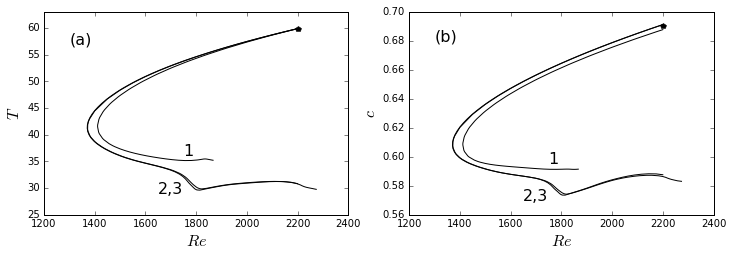
\includegraphics[width=0.9\linewidth]{local_contin.png}}
\caption{Продолжение решения, соответствующего модельному порыву, по числу Рейнольдса: (а) зависимость временного периода $T$ и (b) скорости перемещения порыва вдоль трубы $c$ от числа Рейнольдса $\Re$. Кривые 1, 2 и 3 соответствуют решениям, полученным на различных расчетных сетках, описанных в разделе \ref{edge_seq}. Черные точки соответствует исходному решению, принадлежащему сепаратрисе.}
\label{local_contin_pic}
\end{figure}

Решения с верхней ветви сохраняют пространственно локализованную структуру, но в сравнении с решениями с нижней ветви, имеют большую амплитуду колебаний, большую интенсивность поперечного движения, больший дефект скорости на оси трубы. Скорость перемещения локализованной структуры вдоль трубы для решений, принадлежащих верхней ветви, оказывается ниже. По всем этим параметрам решения, принадлежащие верхней ветви, оказываются ближе к турбулентному порыву, чем решения, принадлежащие нижней ветви. Это дает основания полагать, что и другие результаты, полученные при изучении решений, принадлежащих верхней ветви, также имеют большее отношение к турбулентному порыву. В решении, принадлежащем верхней ветви, $\Re = 1700$, скорость перемещения локализованной структуры вдоль трубы составляется $0.59U$. Скорость перемещения локализованной структуры в исходном решении, принадлежащем нижней ветви, (модельном порыве) составляет $0.69U$. Скорость перемещения турбулентного порыва приблизительно равна $0.5U$. Временной период решения, принадлежащего верхней ветви, $\Re = 1700$, составляет $34.4 R/U$, что почти в два раза меньше, чем у модельного порыва ($59.6R/U$). 

\section{Исследование верхней ветви порожденного модельным порывом семейства условно-периодических решений}

\begin{figure}
\center{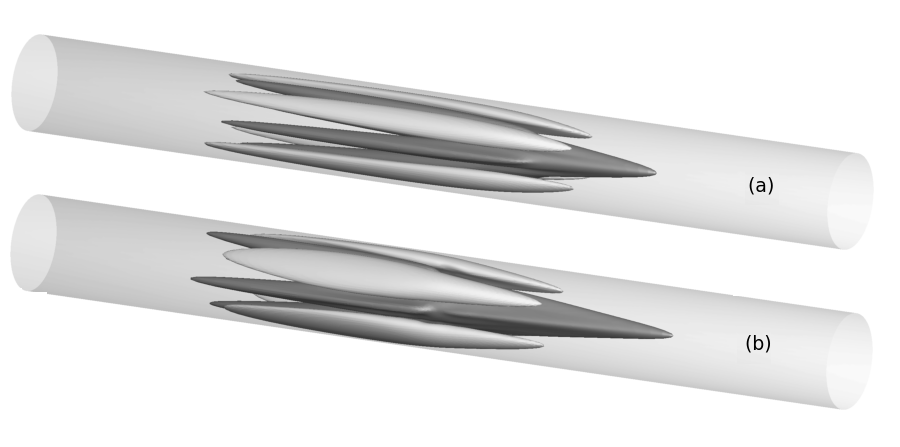
\includegraphics[width=0.9\linewidth]{3D_contin_cmp.png}}
\caption{Среднее поле скорости исходного решения (a) и решения, принадлежащего верхней ветви, $\Re=1700$, (b). Темным и светлым тоном приведены поверхности скорости $-0.1$ и $+0.1$ относительно скорости течения Пуазейля. Поток направлен слева направо.}
\label{3D_contin_cmp_pic}
\end{figure}

Также, как при исследовании модельного порыва, полученного на сепаратрисе, поле скорости $\v_\mathrm{ub}$ модельного порыва, принадлежащего верхней ветви, $\Re = 1700$, представляется в виде суммы средней $\V_\mathrm{ub} = \overline{\v_\mathrm{ub}}^t$ и пульсационной $\v_\mathrm{n,ub} = \v_\mathrm{ub} - \V_\mathrm{ub}$ составляющих; осреднение выполняется по времени в сопутствующей системе отсчета (<<ub>> --- <<up branch>>). Среднее поле скорости $\V_\mathrm{ub}$ представлено на рисунке \ref{3D_contin_cmp_pic} (b). На рисунке (a) для сравнения представлено среднее поле скорости исходного решения (модельного порыва). Качественно структура решения не меняется, среднее поле скорости в обоих случаях содержит полосы повышенной и пониженной скорости, вытянутые вдоль стенки. Полосы пониженной скорости объединяются в передней части порыва в приосевой области, формируя центральное ядро пониженной скорости. В случае решения с верхней ветви ядро пониженной скорости имеет большую протяженность, в то время как пристенные полосы оказываются короче. Суммарная длина структуры при этом практически не меняется. 


\begin{figure}
\center{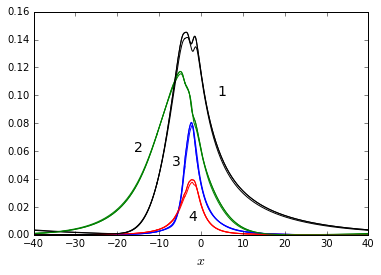
\includegraphics[width=0.6\linewidth]{amp_ub.png}}
\caption{Распределение вдоль трубы амплитуды компонент решения, принадлежащего верхней ветви, $\Re = 1700$: кривая 1 --- $\V_\mathrm{2D,ub}$ (отклонение от течения Пуазейля), кривые 2,4 --- продольная и поперечная компоненты $\V_\mathrm{3D,ub}$, кривая 3 --- амплитуда $\v_\mathrm{n,ub}$. Представлены результаты, полученные на трех расчетных сетках, описанных в разделе \ref{edge_seq}.}
\label{amp_ub_pic}
\end{figure}


На рисунке \ref{amp_ub_pic} изображена средняя по сечению трубы амплитуда различных компонент движения. Как при исследовании модельного порыва, стационарная составляющая движения разделена на двумерную $\V_\mathrm{2D,ub} = \overline{\V_\mathrm{ub}}^{\theta}$ и трехмерную $\V_\mathrm{3D,ub} = \V_\mathrm{ub} - \V_\mathrm{2D,ub}$ составляющие. Продольная и поперечная компоненты трехмерной составляющей движения ассоциируются с полосами и продольными вихрями, соответственно. Качественно, распределение интенсивности различных компонент движения вдоль трубы в рассматриваемом решении, принадлежащем верхней ветви, и в модельном порыве совпадают (см. рис. \ref{amp_pic}), но все компоненты движения в решении, принадлежащем верхней ветви, имеют большую амплитуду. Амплитуда полосчатого движения и пульсаций выше примерно в два раза. Интенсивность продольных вихрей выше почти в четыре раза. На рисунке \ref{amp_ub_pic} представлены результаты, полученные на трех различных расчетных сетках. Параметры расчетных сеток приведены в разделе \ref{edge_seq}. Результаты, полученные на различных сетках, совпадают качественно и близки количественно, что позволяет говорить об адекватности воспроизведения решения в расчетах. 


\begin{figure}
\center{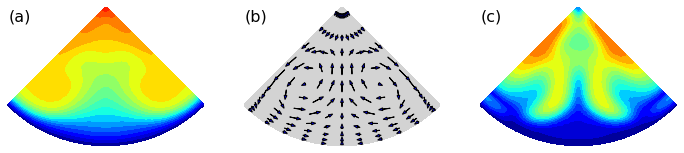
\includegraphics[width=0.9\linewidth]{local_ub_means.png}} 
\center{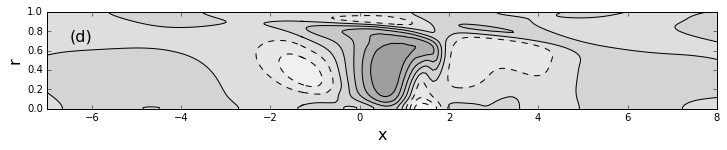
\includegraphics[width=0.9\linewidth]{local_ub_vel1.png}}
\caption{Поле скорости решения, принадлежащего верхней ветви, $\Re = 1700$: в сечении, где пульсации достигают наибольшей амплитуды, приведены изолинии $V_\mathrm{x,ub}$ (a), векторное поле $(V_\mathrm{r,ub}, V_\mathrm{\theta,ub})$ (b), линии равного уровня амплитуды $\v_\mathrm{n,ub}$ (c); в сечении $\theta = 0$ --- изолинии продольной компоненты $\v_\mathrm{n,ub}$ (d). Сплошные линии --- положительные значения, прерывистые --- отрицательные.}
\label{local_ub_means_pic}
\end{figure}

На рисунке \ref{local_ub_means_pic}(a) приведена продольная компонента стационарной составляющей движения $V_\mathrm{x,ub}$ в сечении трубы, где пульсации достигают максимума. В сравнении с исходным решением в решении, принадлежащем верхней ветви, между полосами повышенной и пониженной скорости существуют области, в которых продольная скорость с ростом $r$ (при постоянных $x$ и $\theta$) падает не монотонно. Полосы формируются за счет <<лифт-ап>> эффекта. Векторное поле поперечной компоненты среднего течения $(V_\mathrm{r,ub}, V_\mathrm{\theta,ub})$, приведенное на рисунке (b), соответствует наличию стационарных продольных вихрей между полосами повышенной и пониженной скорости, ответственных за поддержание существования этих полос. На рисунке (с) приведена амплитуда пульсационной составляющей движения $\v_\mathrm{n,ub}$. Пульсации в решении, принадлежащем верхней ветви, имеют более сложную форму, чем в исходном решении, но они также оказываются сконцентрированы между полосой повышенной скорости и осью трубы и между соседними полосами повышенной и пониженной скорости. Форма пульсационной составляющей движения близка к бегущей волне, имеющей в системе отсчета порыва положительную фазовую скорость. Также, как и в модельном порыве, длину этой бегущей волны можно оценить в $5R$. Мгновенное поле скорости пульсационной составляющей движения в продольном сечении трубы $\theta = 0$ приведено на рисунке~(d).  


\begin{figure}
\center{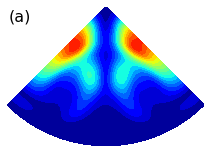
\includegraphics[width=0.3\linewidth]{ub_lin_cs.png} 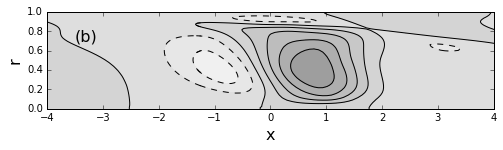
\includegraphics[width=0.6\linewidth]{ub_lin_ls.png}}
\caption{Наиболее быстрорастущее решение линейной задачи устойчивости поля скорости $\V_\mathrm{ub}$:  (а) --- линии уровня амплитуды колебаний в поперечном сечении трубы, где амплитуда колебаний достигает максимума, (b) --- мгновенное поле скорости в сечении $\theta = 0$. Сплошные линии --- положительные значения, прерывистые --- отрицательные.}
\label{ub_lin_pic}
\end{figure}

Также, как в модельном порыве, в решении, принадлежащем верхней ветви, $\Re = 1700$, среднее поле скорости оказывается линейной неустойчиво. Наиболее быстрорастущее решение $\v'_\mathrm{1,ub}$ линейной задачи устойчивости поля скорости $\V_\mathrm{ub}$ воспроизводит форму пульсационной составляющей движения $\v_\mathrm{n,ub}$ и период её изменения во времени, что говорит о том, что пульсационная составляющая движения $\v_\mathrm{n,ub}$ возникает в результате линейной неустойчивости среднего течения. Временной период и инкремент нарастания $\v'_\mathrm{1,ub}$ равны $31.8R/U$ и $0.012U/R$. Временной период $\v_\mathrm{n,ub}$ равен $34.4R/U$. На рисунке \ref{ub_lin_pic}(a) в том же сечении, в котором пульсационная составляющая движения представлена на рисунке \ref{local_ub_means_pic}(c), приведена средняя по времени амплитуда колебаний в решении $\v'_\mathrm{1,ub}$. Распределение амплитуды колебаний для решения линеаризованных и решения полных уравнений достаточно точно совпадают. В $\v'_\mathrm{1,ub}$ колебания также оказываются сконцентрированы между полосой повышенной скорости и осью трубы и между соседними полосами повышенной и пониженной скорости. Мгновенное поле продольной компоненты $\v'_\mathrm{1,ub}$, представленное в продольном сечении $\theta = 0$ на рисунке \ref{ub_lin_pic}(b), также демонстрирует согласие с мгновенным полем скорости $\v_\mathrm{n,ub}$, приведенным на рисунке \ref{local_ub_means_pic}(d). В области расположения полосы повышенной скорости вдоль потока друг за другим следуют области повышенной и пониженной скорости. Суммарная протяженность одной области повышенной скорости и одной области пониженной скорости составляет приблизительно $5R$. Общая протяженность области, в которой пульсации имеют существенную амплитуду, равна примерно $5$--$7R$. По форме пульсации близки к бегущей волне, что согласуется с тем, что они возникают в результате линейной неустойчивости среднего течения, слабо меняющегося вдоль трубы. Отметим, что поле скорости $(V_\mathrm{x,ub}, 0, 0)$ оказывается линейно устойчивым, соответствующий инкремент затухания равен $\lambda = -0.009U/R$. 


\begin{figure}
\center{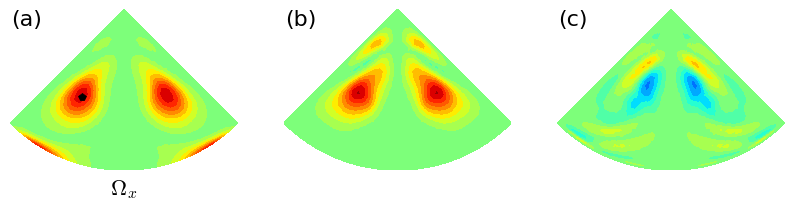
\includegraphics[width=0.9\linewidth]{ub_OXgen_map.png}}
\caption{Механизм поддержания стационарных продольных вихрей в условно периодическом решении, принадлежащем верхней ветви, $\Re = 1700$: в сечении трубы, где пульсации достигают наибольшей амплитуды, приведены линии уровня $\Omega_x^2$ (a), вклад в поддержание $\Omega_x^2$ со стороны слагаемых, соответствующих \eqref{time_OXgen_terms} (b) и сумме других слагаемых в правой части \eqref{time_OX_eq} (c). Сплошные линии --- положительные значения, прерывистые --- отрицательные.}
\label{ub_OXgen_pic}
\end{figure}


Механизмы поддержания стационарных продольных вихрей в решении, принадлежащем верхней ветви, и в модельном порыве также согласуются. На рисунке \ref{ub_OXgen_pic}(a) приведен квадрат стационарной продольной завихренности $\Omega_\mathrm{x, ub}^2$ в сечении трубы, где амплитуда пульсаций достигает наибольшей величины. Распределение $\Omega_\mathrm{x,ub}^2$ по сечению трубы соответствует наличию пары продольных вихрей, расположенных между полосами повышенной и пониженной скорости (см. рис. \ref{local_ub_means_pic}(b)). На рисунках \ref{ub_OXgen_pic}(b,c) приведены значения слагаемых \eqref{time_OXgen_terms} и других слагаемых из правой части уравнения \eqref{time_OX1_eq}, умноженные на $2\Omega_\mathrm{x,ub}$. Умножение слагаемых из правой части уравнения \eqref{time_OX1_eq} на $2\Omega_\mathrm{x,ub}$ дает вклад этих слагаемых в поддержания поля $\Omega_\mathrm{x,ub}^2$. Слагаемые \eqref{time_OXgen_terms} определяют форм поля стациоанрной продольной завихренности, вклад других слагаемых в правой части \eqref{time_OX1_eq} оказывается отрицательным. Нет сомнения, что за образование стационарных продольных вихрей в уравнении \eqref{time_OX1_eq} ответственны слагаемые \eqref{time_OXgen_terms}. Дополнительно, на рисунке \ref{ub_oxgen_lines_pic}(a) приведено значение $\Omega_x^2$ и слагаемых, отвечающих за его формирование, на прямой, проходящей через область, занятую положительным вихрем, $r = 0.6, \theta = \pi/10$. Картина течения в этом случае значительно сложнее, чем в модельном порыве (см. рис. \ref{xline_oxgen_pic}(a)). Тем не менее, графики на рисунке \ref{ub_oxgen_lines_pic}(a) также подтверждают представление о том, что за образование продольных вихрей ответственно слагаемое \eqref{time_OXgen_terms}. 
 

\begin{figure}
\center{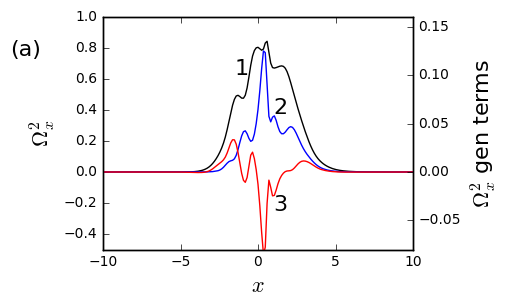
\includegraphics[width=0.5\linewidth]{ub_OXgen_lines.png}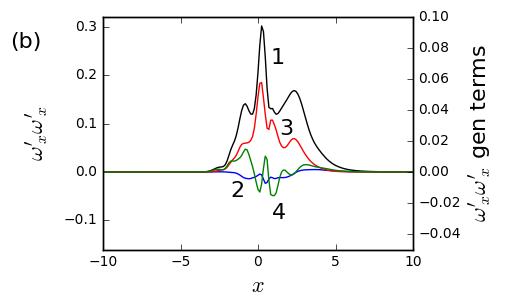
\includegraphics[width=0.5\linewidth]{ub_ox1gen_lines.png}}
\caption{Механизм поддержания продольных вихрей в условно периодическом решении, принадлежащем верхней ветви, $\Re = 1700$. На прямой, проходящей через область, занятую положительным вихрем, $r = 0.6$, $\theta = \pi/10$, приведены значения: (a) --- $\Omega_x^2$ (кривая 1) и вклад в поддержание $\Omega_x^2$ со стороны слагаемых, соответствующих \eqref{time_OXgen_terms} (кривая 2) и другим слагаемым в правой части \eqref{time_OX1_eq} (кривая 3); (b) --- $\overline{\omega'_x\omega'_x}^t$ (кривая 1) и вклад в её поддержание со стороны слагаемых, соответствующих \eqref{time_ox1gen_term2} (кривая 2) и другим слагаемым в правой части уравнения \eqref{time_ox1_eq} (кривая~3).} 
\label{ub_oxgen_lines_pic}
\end{figure}


То, что слагаемые \eqref{time_OXgen_terms} не равны нулю, говорит о наличии согласованности между пульсациями продольной скорости и пульсациями продольной завихренности. Объяснить наличие согласованности позволяет механизм образования пульсаций продольной завихренности. Механизмы образования пульсаций продольной завихренности в рассматриваемом решении и в модельном порыве также согласуются. В уравнении \eqref{time_ox2_eq}, описывающем эволюцию пульсаций продольной завихренности $\omega'_\mathrm{x,ub}$, за образование $\omega'_\mathrm{x,ub}$ в области расположения продольных вихрей отвечает слагаемое \eqref{time_ox1gen_term2}. На рисунке \ref{ub_oxgen_lines_pic}(b) также, как на рисунке (a), приведено значение амплитуды пульсационной составляющей движения $\overline{\omega'_\mathrm{x,ub}\omega'_\mathrm{x,ub}}^t$ и вкладов в её образование со стороны слагаемых \eqref{time_ox1gen_term2} и других слагаемых в правой части уравнения \eqref{time_ox2_eq}. Вклад слагаемых уравнения \eqref{time_ox2_eq} в поддержание $\overline{\omega'_\mathrm{x,ub}\omega'_\mathrm{x,ub}}^t$ получен их домножением на $2\omega'_\mathrm{x,ub}$ с последующим осреднением по времени. Слагаемое \eqref{time_ox1gen_term2} дает определяющий вклад в производство  $\overline{\omega'_\mathrm{x,ub}\omega'_\mathrm{x,ub}}^t$ в то время, как другие слагаемые в правой части уравнения \eqref{time_ox2_eq} оказываются преимущественно отрицательное влияние. Механизм образования пульсаций продольной завихренности, выраженный слагаемым \eqref{time_ox1gen_term2}, состоит в сжатии и растяжении вихревых нитей, соответствующих стационарным продольным вихрям, пульсациями продольной скорости. Детали механизма образования стационарных продольных вихрей и пульсаций продольной завихренности приведены в разделе \ref{edge_oxgen}.

Таким образом, продолжив модельный порыв по числу Рейнольдса, удалось достичь точки бифуркации, в которой рождаются две ветви решений, и перейти с нижней ветви на верхнюю. Двигаясь по верхней ветви решений в сторону увеличения числа Рейнольдса удалось получить новые условно периодические решения с пространственно-локализованной структурой, по ряду качественных характеристик оказывающихся ближе к турбулентному порыву, чем исходное решение. Были описаны основные характеристики решения с верхней ветви и механизм поддержания колебаний в нем. Все основные элементы цикла поддержания колебаний в решении, принадлежащем верхней ветви, и в модельном порыве совпадают. Периодичность решения по времени в сопутствующей системе отсчета позволяет разделить его поле скорости на среднюю и пульсационную составляющие осреднением по времени. Показано, что пульсационная составляющая движения возникает в результате линейной неустойчивости среднего течения. В среднем течении выделяются полосы повышенной и пониженной скорости, вытянутые вдоль потока. Пульсации оказываются сконцентрированы между полосами повышенной и пониженной скорости, где в среднем течении находятся точки перегиба, если рассматривать его как функцию угловой координаты. Вероятно, механизм образования пульсаций является механизмом типа Кельвина--Гельмгольца. В потоке существуют стационарные продольные вихри, поддерживающие существование полос. Существование продольных вихрей, в свою очередь, поддерживается нелинейным взаимодействием пульсаций продольной скорости и пульсаций продольной завихренности. В области расположения продольных вихрей пульсации продольной завихренности образуются за счет сжатия и растяжения существующих вихревых нитей пульсациями продольной скорости. Таким образом, формируется необходимая для поддержания продольных вихрей согласованность между пульсациями продольной скорости и пульсациями продольной завихренности. 

\section{Семейство трехмерных бегущих волн в течении Гагена-Пуазейля} \label{pipeTW_seq}

Решение уравнений Навье-Стокса, соответствующее модельному порыву, является предельным состоянием решения, эволюционирующего на сепаратрисе, разделяющей в фазовом пространстве области притяжения решений, соответствующие ламинарному и турбулентному режимам течения. В согласии с \cite{Avila2013}, при дополнительном условии $5R$ периодичности вдоль потока предельное решение на сепаратрисе имеет еще более простое пространственно-временное поведение, а именно, имеет вид бегущей волны. Как показано в разделе \ref{pipe_tw_seq}, это решение в более простой форме воспроизводит все основные элементы цикла поддержания колебаний, выделенные при изучении модельного порыва. Среднее поле скорости бегущей волны не зависит от продольной координаты, благодаря чему полосы повышенной и пониженной скорости и продольные вихри в бегущей волне имеют бесконечную протяженность, в то время как в модельном порыве их протяженность ограничена. 

\begin{figure}
\center{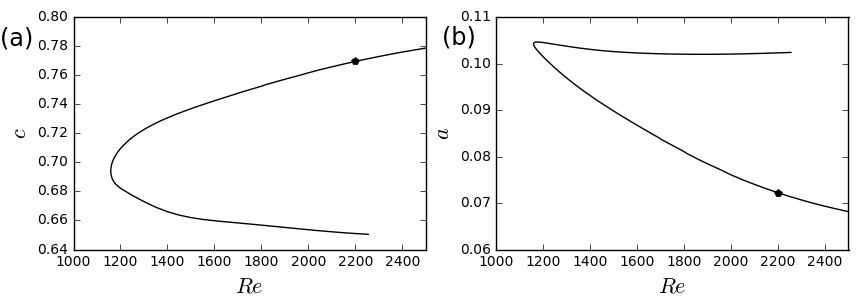
\includegraphics[width=0.9\linewidth]{pipeTW-contin.png}}
\caption{Продолжение решения уравнений Навье-Стокса, имеющего вид бегущей волны, по числу Рейнольдса: (а) зависимость фазовой скорости и (b) амплитуды трехмерной составляющей движения от числа Рейнольдса. Точка соответствует исходному решению, найденному на сепаратрисе.} 
\label{pipeTW_contin_pic}
\end{figure}

Продолжение по числу Рейнольдса решения, имеющего вид бегущей волны, найденного на сепаратрисе, позволило получить новые решения в виде бегущей волны. На рис. \ref{pipeTW_contin_pic} приведены значения фазовой скорости $c_\mathrm{tw}$ и средней по объему трубы амплитуды трехмерной составляющей движения $\V_\mathrm{3D} = \v - \overline{\v}^{x,\theta}$. Как и условно периодические решения, порожденные модельным порывом, решения в виде бегущей волны принадлежат однопараметрическому множеству. Семейство решений, порожденное бегущей волной, найденной на сепаратрисе, возникает в результате бифуркации при $\Re \approx 1200$. При меньших числах Рейнольдса решений из этого семейства не существует. При больших числах Рейнольдса существует две ветви решений. В точке бифуркации производная по числу Рейнольдса от характеристик решения обращается в бесконечность, что не позволяет перейти с одной ветви решения на другую, продлевая решение по числу Рейнольдса. Для того, чтобы перейти с одной ветви решения на другу, вблизи от точки бифуркации продолжение решения было выполнено по фазовой скорости $c_\mathrm{tw}$. Число Рейнольдса, при этом, было включено в число определяемых параметров. Ветвь, которой принадлежит исходное решение, найденное на сепаратрисе, принято называть нижней, так как для нее характерна меньшая интенсивность колебаний (см. рис. \ref{pipeTW_contin_pic}(b)). Решения с верхней ветви по амплитуде колебаний оказываются ближе к турбулентному течения, что делает их привлекательными для исследования. 

\begin{figure}
\center{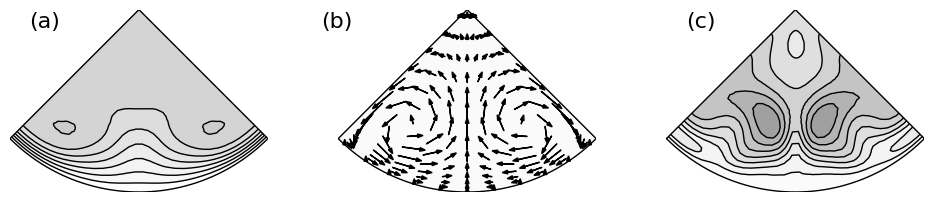
\includegraphics[width=1\linewidth]{pipeTW-1700ub-means.png}}
\center{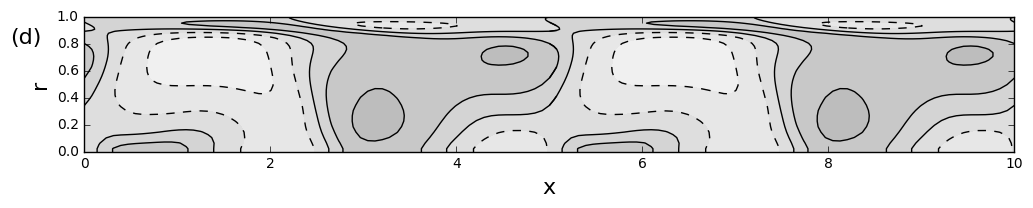
\includegraphics[width=1\linewidth]{pipeTW-1700ub-puls.png}}
\caption{Поле скорости решения, имеющего вид бегущей волны, принадлежащего верней ветви, $\Re = 1700$: (a) --- изолинии средней продольной скорости, (b) --- средняя поперечная скорость, (c) --- линии уровня амплитуды пульсаций, (d) --- изолинии продольной компоненты пульсационной составляющей движения в сечении $\theta = 0$ (продольный период $L_x = 5$). Сплошные линии --- положительные значения, прерывистые -- отрицательные. } 
\label{pipeTWub_means_pic}
\end{figure}

Исходная сетка, на которой были найдены решения, содержит $32 \times 32 \times 32$ ячеек в продольном, радиальном и угловом направлениях. Протяженность расчетной области составляет $L_x = 5R$. Для того, чтобы установить влияние расчетной сетки на результат, решения были пересчитаны на более подробной сетке, содержащей вдвое большее число ячеек в каждом направлении ($64 \times 64 \times 64$). Разрешение расчетных сеток, на которых получены решения в виде бегущих волн, точно совпадает с разрешением сеток, на которых получен модельный порыв (см. раздел \ref{edge_seq}). Для адекватного воспроизведения решений с верхней ветви требуются более подробные расчетные сетки, чем для решений с нижней ветви. Расчеты, проведенные на двух расчетных сетках, показали, что до $\Re \approx 2000$ решение на верхней ветви воспроизводится адекватно. Также, как при исследовании верхней ветви семейства решений, порожденного модельным порывом, характеристики верхней ветви решений, имеющих вид бегущей волны, будут представлены на примере решения с $\Re = 1700$. Это решение оказывается устойчивым (при наложенных дополнительных условиях симметрии \eqref{sym_eq}, \eqref{per_eq}, \eqref{bc2_eq}). Его фазовая скорость равна $c_\mathrm{tw,ub} = 0.66U$. 

\begin{figure}
\center{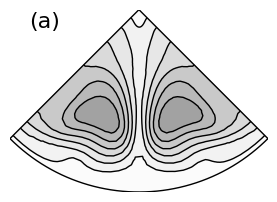
\includegraphics[width=0.33\linewidth]{pipeTW-1700ub-lin-map.png} 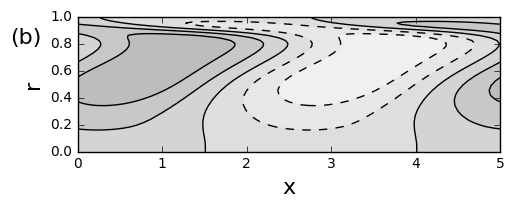
\includegraphics[width=0.6\linewidth]{pipeTW-1700ub-lin-puls.png}}
\caption{Наиболее быстро растущее собственное решение линейной задачи устойчивости поля скорости $\V_\mathrm{tw,ub}$: (a) --- линии уровня амплитуды колебаний; (b) --- изолинии продольной компоненты скорости в сечении $\theta = 0$. Сплошные линии --- положительные значения, прерывистые --- отрицательные.}
\label{pipeTWub_lin_pic}
\end{figure}

Также, как при анализе бегущей волны, найденной на сепаратрисе, выполненном в разделе \ref{pipe_tw_seq}, разделим поле скорости выбранной для анализа бегущей волны $\v_\mathrm{tw,ub}$ на среднюю $\V_\mathrm{tw,ub} = \overline{\v_\mathrm{tw,ub}}^x$ и пульсационную $\v'_\mathrm{tw,ub} = \v_\mathrm{tw,ub} - \V_\mathrm{tw,ub}$ составляющие путем осреднения в продольном направлении, обозначенного чертой над выражением с индексом $x$.  Для бегущей волны осреднение в продольном направлении эквивалентно осреднению по времени (при условии, что оно выполнено в системе отсчета, скорость перемещения которой не совпадает с фазовой скоростью волны). Среднее поле скорости зависит только от двух координат, $r$ и $\theta$, что делает его удобным объектом для исследования. 

Также, как и в других исследованных решениях, среднее поле скорости включает полосы повышенной и пониженной скорости, вытянутые вдоль потока. Распределение средней продольной скорости приведено на рис. \ref{pipeTWub_means_pic}(а). В центральной части расчетной области, где медленная жидкость проникает ближе к центру трубы, находится полоса пониженной скорости. При большем и меньшем значении $\theta$ находятся полосы повышенной скорости. Отметим, что скорость жидкости в области расположения полос повышенной скорости оказывается даже выше, чем на оси трубы. Существование полос поддерживается слабым движением жидкости в нормальной к основному потоку плоскости. Распределение средней поперечной скорости, приведенное на рис. \ref{pipeTWub_means_pic}(b), соответствует наличию продольных вихрей, поддерживающих существование полос. Там, где медленная жидкость движется от стенки, находятся полосы пониженной скорости. Там, где жидкость движется ближе к стенке --- полосы повышенной скорости. 

\begin{figure}
\center{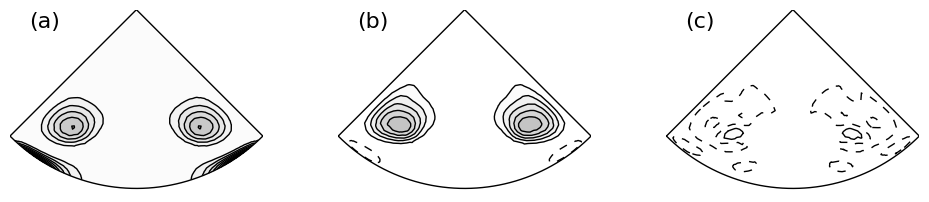
\includegraphics[width=1\linewidth]{pipeTW-1700ub-OXgen.png}}
\caption{Образование продольных вихрей в решении, имеющем вид бегущей волны, принадлежащем верхней ветви, $\Re = 1700$: значение $\Omega_x^2$ (a), вклад в генерацию $\Omega_x^2$ со стороны слагаемых, соответствующих слагаемым \eqref{OXgen_terms} (b) и другим слагаемым в правой части \eqref{OX_eq} (с). Сплошные линии --- положительные значения, прерывистые --- отрицательные.}
\label{pipeTWub_OXgen_pic}
\end{figure}

Пульсации оказываются сосредоточены между полосами повышенной и пониженной скорости и, в несколько меньшей степени, в области расположения полос повышенной скорости (см. рис. \ref{pipeTWub_means_pic}(c)). Отметим, что распределения средней скорости и пульсаций в этом случае значительно отличаются от аналогичных распределений для решения с верхней ветви семейства решений, порожденного модельным порывом (см. рис. \ref{local_ub_means_pic}). В решении, порожденном модельным порывом, скорость на оси трубы оказывается выше, чем в полосах повышенной скорости, пульсации достигают максимума между полосами повышенной скорости и осью трубы, интенсивность пульсаций между полосами разных знаков оказывается значительно ниже. По-видимому, это объясняется наличием продольной неоднородность в пространственно-локализованном решении. 

Мы полагаем, что механизм образования пульсаций в случае рассматриваемой бегущей волны также, как и в других случаях, является линейным. Хотя среднее поле скорости $\V_\mathrm{tw,ub}$ оказывается линейно устойчивым, собственная функция, соответствующая наиболее медленно затухающему собственному решению, $\v'_1$ повторяет форму пульсационной составляющей движения и скорость ее перемещения вдоль трубы. Амплитуда колебаний $\v'_1$ приведена на рис. \ref{pipeTWub_lin_pic}(a). Как и в пульсационной составляющей движения, колебания $\v'_1$ оказываются сосредоточены между полосами повышенной и пониженной скорости, а также, от части, в области расположения полос повышенной скорости. Распределения мгновенной продольной скорости, приведенные для пульсационной составляющей движения $\v'_\mathrm{tw,ub}$ на рис. \ref{pipeTWub_means_pic}(d), а для $\v'_1$ на рис. \ref{pipeTWub_lin_pic}(b), также согласуются друг с другом. Фазовая скорость $\v'_1$ равна $c_1 = 0.63$, декремент затухания $\lambda_1 = -0.0085$. Линейная устойчивость среднего течения не противоречит тому, что механизм передачи энергии в пульсационную составляющую движения является линейный. Амплитуда колебаний в рассматриваемом решении оказывается достаточно велика и достигает $0.15$. Полосы повышенной и пониженной скорости в решении смещаются в боковом направлении с достаточно существенной амплитудой, в результате чего среднее течение недостаточно точно воспроизводит форму полос --- угловые градиенты продольной скорости в среднем течении оказываются ниже, чем в неосредненном поле скорости $\v_\mathrm{tw,ub}$, и скорость роста возмущений на среднем поле скорости может оказаться ниже, чем на неосредненном.

\begin{figure}
\center{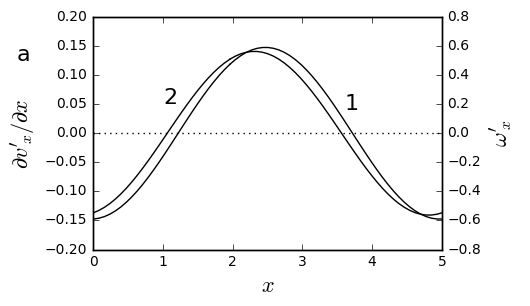
\includegraphics[width=0.5\linewidth]{pipeTW-1700ub-corrA.png}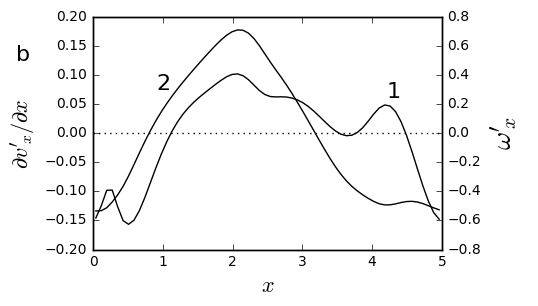
\includegraphics[width=0.5\linewidth]{pipeTW-1700ub-corrB.png}}
\caption{Значения $\d v_x' /\d x$ (кривая 1) и $\omega_x'$ (кривая 2) на прямой, где $\Omega_x$ достигает максимума, $r = 0.75, \theta = \pi/10$: (a) --- для пульсаций, полученных в линейном приближении; (b) --- для пульсационной составляющей движения. }
\label{pipeTWub_corr_pic}
\end{figure}

Существование продольных вихрей, формирующих полосы повышенной и пониженной скорости, объясняется наличием пульсаций. Продольным вихрям, имеющим различные направления вращения, соответствуют области концентрации положительной и отрицательной средней продольной завихренности $\Omega_x$. Как и в других исследованных решениях, в рассматриваемом решении в уравнении баланса средней продольной завихренности \eqref{OX1_eq} за образование продольных вихрей ответственны слагаемые \eqref{OXgen_terms}, описывающие нелинейное взаимодействие пульсаций продольной скорости и пульсаций продольной завихренности. Работать удобнее с уравнением баланса квадрата средней продольной завихренности $\Omega_x^2$, получаемым умножением уравнения \eqref{OX1_eq} на $2\Omega_x$. Положительное значение источниковых членов в этом уравнении говорит об их положительном вкладе, а отрицательное значение --- об отрицательном. Значение слагаемых \eqref{OXgen_terms}, умноженных на $2\Omega_x$, приведено на рис. \ref{pipeTWub_OXgen_pic}(b). Значение суммы других слагаемых в правой части \eqref{OX1_eq}, умноженных на $2\Omega_x$, приведено на рис. \ref{pipeTWub_OXgen_pic}(c). Слагаемые \eqref{OXgen_terms} определяют форму поля $\Omega_x$ в области расположения продольных вихрей, другие источниковые слагаемые дают преимущественно отрицательный вклад в подержание продольной завихренности и по амплитуде значительно уступают выделенному слагаемому. Таким образом, нет сомнений, что и в этом случае за образование продольных вихрей отвечают слагаемые \eqref{OXgen_terms}. Пульсации, полученные в рамках линеаризованных уравнений, $\v_1$ также воспроизводят описанный механизм образования продольных вихрей, но имеют более простую форму (их поле скорости меняется вдоль трубы по гармоническому закону), что делает их привлекательным объектом для анализа. 

\begin{figure}[h]
\center{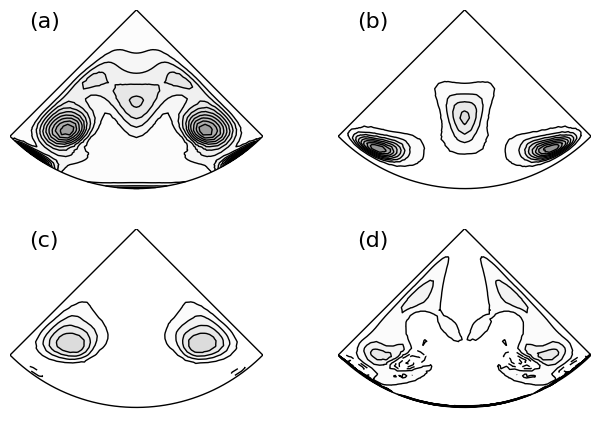
\includegraphics[width=0.66\linewidth]{pipeTW-1700ub-ox1gen.png}}
\caption{Образование пульсаций продольной завихренности в решении, имеющем вид бегущей волны, принадлежащем верхней ветви, $\Re = 1700$: средний квадрат пульсаций продольной завихренности $\overline{\omega'_x \omega'_x }^x$ (а), вклад в производство $\overline{\omega'_x \omega'_x }^x$ слагаемых, соответствующих слагаемым \eqref{ox1gen_add_terms} (b), слагаемому \eqref{ox1gen_main_terms} (c) и сумме остальных слагаемых в правой части \eqref{ox2_eq} (d). Сплошные линии --- положительные значения, прерывистые --- отрицательные.}
\label{pipeTWub_ox1gen_pic}
\end{figure}

Между собой слагаемые \eqref{OXgen_terms} оказываются равны в силу периодичности поля скорости вдоль потока, поэтому мы ограничимся анализом второго из слагаемых. Отличие от нуля этого слагаемого говорит о наличие корреляции между пульсациями продольной скорости и пульсациями продольной завихренности, причем эта корреляция такова, что в области расположения положительного вихря $\omega'_x$ и ${\partial v'_x}/{\partial x}$ имеют положительную корреляцию, а в области расположения отрицательного вихря --- отрицательную, что позволяет поддерживать существование этих вихрей. Для того, чтобы продемонстрировать наличие корреляции, на рис. \ref{pipeTWub_corr_pic} приведено значение $\omega'_x$ и ${\partial v'_x}/{\partial x}$ на прямой, параллельной оси $x$, проходящей через центр положительного вихря, $r = 0.75, \theta = \pi/10$. На рисунке (a) приведены значения для пульсаций, полученных в рамках линеаризованных уравнений, $\v'_1$. Кривые меняются вдоль потока по гармоническому закону и оказываются в фазе друг с другом, что обеспечивает наибольшую эффективность производства $\Omega_x$. На рисунке (b) приведены аналогичные значения для пульсационной составляющей движения $\v'_\mathrm{tw,ub}$. Хотя в сравнении с линейным случаем или со случаем аналогичного решения с нижней ветви (см. рис. \ref{OXgen_corr_pic}) графики имеют значительно более сложную форму, между ними также имеется существенная корреляция (кривые достигают наибольшего и наименьшего значения в близких точках). Наличие корреляции объясняет механизм образования пульсаций продольной завихренности $\omega'_x$, общий во всех рассматриваемых решениях.

В уравнении \eqref{ox2_eq} за образование пульсаций продольной завихренности $\omega'_x$ в области расположения продольных вихрей ответственно слагаемое \eqref{ox1gen_main_terms}, отписывающее эффект сжатия и растяжения существующих в потоке вихревых трубок, вызванного пульсациями продольной скорости. Для того, чтобы продемонстрировать вклад слагаемого \eqref{ox1gen_main_terms} в образование $\omega'_x$, обратимся к уравнению баланса среднего квадрата пульсаций продольной завихренности $\overline{\omega'_x\omega'_x}^x$, полученного умножением \eqref{ox2_eq} на $2\omega'_x$ с последующим определением по $x$. Слагаемые в этом уравнении зависят только от $r$ и $\theta$, положительное значение источниковых членов в этом уравнении говорит об их содействии образованию $\omega'_x$, а отрицательное --- о противодействии. На рис. \ref{pipeTWub_ox1gen_pic} приведено значение $\overline{\omega'_x\omega'_x}$ (a) и вклада в его образование со стороны слагаемых, соответствующих \eqref{ox1gen_add_terms}, (b), слагаемого, соответствующего \eqref{ox1gen_main_terms}, (c) и слагаемых, соответствующих сумме других слагаемых в правой части уравнения \eqref{ox2_eq}. Наибольший вклад в образование $\omega'_x$ дают слагаемые \eqref{ox1gen_add_terms}, отвечающие за поворот нормальных к стенке вихревых нитей на фоне нормального к стенке градиента скорости. Хотя эти слагаемые имеют существенное значение вблизи области расположения продольных вихрей, они не участвуют в поддержании продольных вихрей, так как пульсации, формируемые этими слагаемыми, согласованы с пульсациями продольной скорости таким образом, что их нелинейное взаимодействие близко к нулю (см. раздел \ref{ox1gen_seq}). Образование пульсаций $\omega'_x$ в области расположения продольных вихрей связано со слагаемым \eqref{ox1gen_main_terms}. Именно это слагаемое обеспечивает необходимую для поддержания продольных вихрей согласованность между пульсациями продольной скорости и пульсациями продольной завихренности. Другие источниковые слагаемые в области расположения продольных вихрей имеют как положительное, так и отрицательное значение, и существенного влияния на образование $\omega'_x$ в интересующей нас области не оказывают. 

Для верхней ветви решений, имеющих вид бегущей волны, механизм образования колебаний оказывается таким же, как и для других исследованных решений за тем исключением, что среднее поле скорости оказывается линейно устойчивым. Тем не менее, эта особенность решения не говорит о том, что механизм передачи энергии в пульсационную составляющую движения отличается от линейного. 



\begin{comment}
Re2200ub:
lin: cf = 0.44473618074359494, lambda = -0.0085
vwz: cf = 0.6470799307435949, lambda = -0.021

Re1700ub:
lin: cf = 0.633021694959945, lambda = -0.02
vwz: cf = 0.651179838899339, lambda = -0.028 (unsym)
        Осесимметричное возмущение, lambda = -0.028
\end{comment}

\section{Семейства трехмерных бегущих волн в плоском течении Пуазейля} \label{ductTW_seq}

В работе исследованы некоторые случаи движения жидкости в плоском канале. Постановка задачи о движении жидкости в плоском канале во многом аналогична постановке задачи о движении жидкости в круглой трубе. Решаются уравнение Навье-Стокса для несжимаемой жидкости \eqref{NS_eq} и уравнение неразрывности \eqref{div_eq} в прямоугольной системе координат; $x, y, z$ --- продольная, нормальная к стенке и поперечная координаты. Полуширина канала равна $H$. На стенках канала $y = 0$ и $y = 2H$ ставится условие прилипания. В направлениях $x$ и $z$ движение считается периодическим. Дополнительно на решение накладываются условия отражения относительно плоскостей $y = H$ и $z = 0$:
\begin{equation} \label{duct_ysym_eq}
(v_x, v_y, v_z)(x, H+y, z) = (v_x, -v_y, v_z)(x, H-y, z),
\end{equation} 
\begin{equation} \label{duct_zsym_eq}
(v_x, v_y, v_z)(x, y, z) = (v_x, v_y, -v_z)(x, y, -z). 
\end{equation} 
Условие \eqref{duct_ysym_eq}, эквивалентное условию проскальзывания на плоскости $y = H$, исключает влияние каждой из стенок на движение жидкости вблизи противоположной стенки. Условие \eqref{duct_zsym_eq} исключает смещение возникающих в потоке структур в направлении~$z$ и фиксирует их положение в пространстве. Расчетная область, таким образом, имеет форму параллелепипеда размера $L_x \times H \times L_z$, где $L_x$ --- период изменения решения в направлении $x$, $L_z$ --- половина периода изменения решения в направлении~$z$. Жидкость приводится в движение продольным градиентом давления, определяемым из условия постоянства расходной скорости $U_m$. Задача решается численно конечно-разностным методом, аналогичным методу, описанному в разделе \ref{num_method}. Число Рейнольдса $\Re = UH/\nu$ вводится через полуширину канала $H$, максимальную скорость в течении Пуазейля $U = 3/2U_m$ и кинематический коэффициент вязкости $\nu$. 

Условия \eqref{duct_ysym_eq} и \eqref{duct_zsym_eq} аналогичны условиям \eqref{sym_eq} и \eqref{per_eq}, примененным при исследовании движения жидкости в круглой трубе. Упрощая поведение решения, эти условия позволяют найти в плоском течении Пуазелйя решения, имеющие вид бегущей волны. Все рассматриваемые в разделе решения получены при $L_x = 5H$. Обнаружено, что при $L_z = 1{,}2H$, $\Re = 2000$ вид бегущей волны имеет предельное состояние решения, эволюционирующего на сепаратрисе. Фазовая скорость бегущей волны равна $c_\mathrm{tw}=0.97U$. Алгоритм поиска решения на сепаратрисе описан в разделе \ref{edge_seq}. Также обнаружено, что при $L_z = H$, $\Re = 1400$ существует устойчивое решение в виде бегущей волны (при наложенных условиях симметрии). Это решение может быть получено прямым интегрированием уравнений движения по времени с некоторыми случайными начальными данными. Его фазовая скорость равна $c_\mathrm{tw} = 0.73U$. Оба решения получены на расчетной сетке, содержащей $64 \times 40 \times 32$ ячеек. В нормальном к стенке направлении введено сгущение сетки таким образом, что высота ячейки вблизи стенки в 4 раза меньше, чем в центре канала. 

\begin{figure}
\center{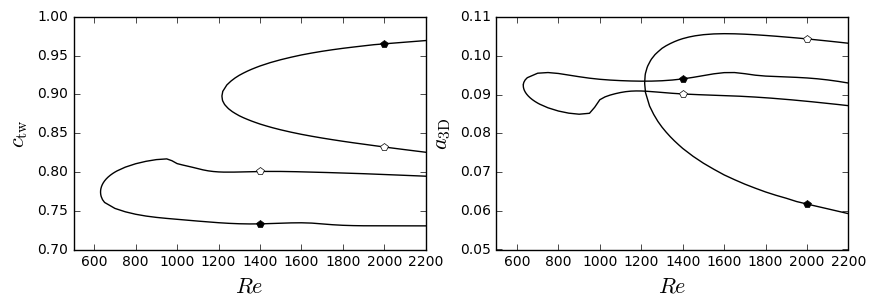
\includegraphics[width=0.9\linewidth]{ductTW-contin.png}}
\caption{Продолжение по числу Рейнольдса решения, найденного на сепаратрисе, (1) и устойчивого решения (2), имеющих вид бегущей волны: зависимость фазовой скорости $c_\mathrm{tw}$ (a) и амплитуды трехмерной составляющей движения $\v_\mathrm{3D}$ (b) от числа Рейнольдса. Точки соответствуют исходным решениям, найденным отличным от продолжения по параметра методом.}
\label{ductTW_contin_pic}
\end{figure}

Продолжение найденных бегущих волн по числу Рейнольдса позволило получить два семейства решений. В процессе продолжения по числу Рейнольдса поле скорости бегущей волны и ее фазовая скорость определяются однозначно --- решения принадлежат однопараметрическому множеству (см. рис. \ref{ductTW_contin_pic}). Обнаружено, что бегущая волна, найденная на сепаратрисе, и устойчивая бегущая волна порождают различные семейства решений. Эти семейства возникают в результате бифуркации при $\Re \approx 1200$ и $\Re \approx 630$ и имеют по две ветви --- нижнюю и верхнюю. Для решений с нижней ветви в сравнении с решениями с верхней ветви характерна большая фазовая скорость и меньшая амплитуда колебаний. Фазовая скорость решений приведена на рис. \ref{ductTW_contin_pic}(a), амплитуда трехмерной составляющей движения $\v_\mathrm{3D} = \v - \overline{\v}^{x,z}$ ---  на рис. \ref{ductTW_contin_pic}(b). Бегущая волна, найденная на сепаратрисе, принадлежит нижней ветви соответствующего семейства (точка на кривой 1), а устойчивая бегущая волна --- верхней (точка на кривой 2). Для того, чтобы составить представление о нижней и верхней ветвях каждого семейства решений, выполним более подробный анализ четырех решений, которые мы будем именовать решениями А, Б, В, Г: бегущей волны, найденной на сепаратрисе, (А) и соответствующей ей бегущей волны с верхней ветви с тем же значением числа Рейнольдса $\Re = 2000$ (Б); устойчивой бегущей волны (Г) и соответствующей ей бегущей волны с нижней ветви с тем же значением числа Рейнольдса $\Re = 1400$ (В). Фазовая скорость бегущих волн Б и В составляет $c_\mathrm{tw} = 0.82U$ и $0.8U$, соответственно. Выбранные для анализа решения существенно отличаются друг от друга, но воспроизводят общие элементы цикла поддержания колебаний. 

\begin{figure}
\center{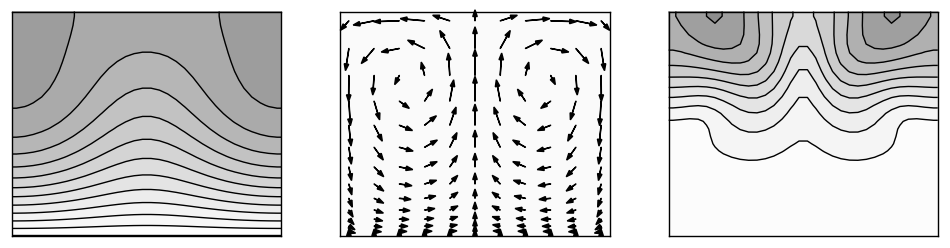
\includegraphics[width=0.9\linewidth]{ductTW-edge2000low-means.png}}
\center{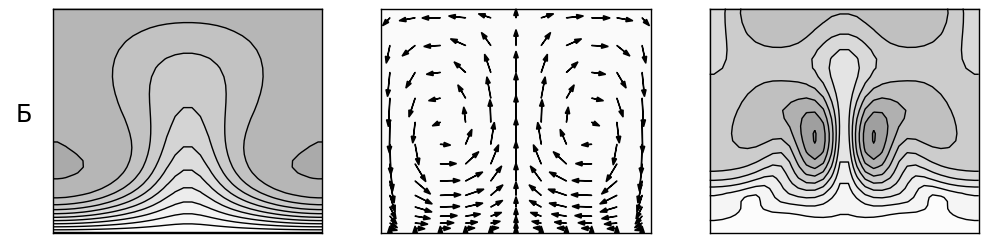
\includegraphics[width=0.9\linewidth]{ductTW-edge2000up-means.png}}
\center{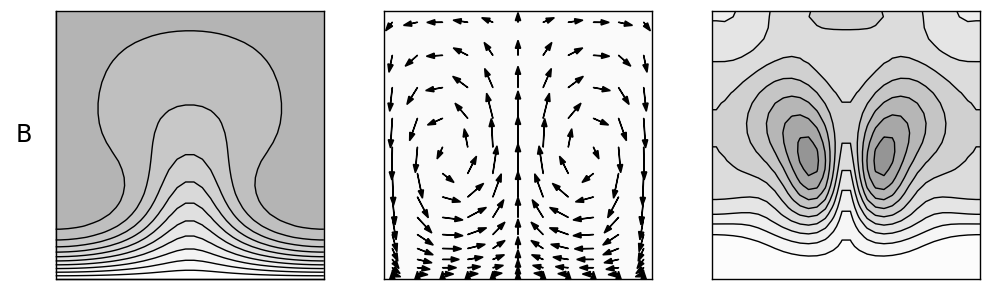
\includegraphics[width=0.9\linewidth]{ductTW-turb1400low-means.png}}
\center{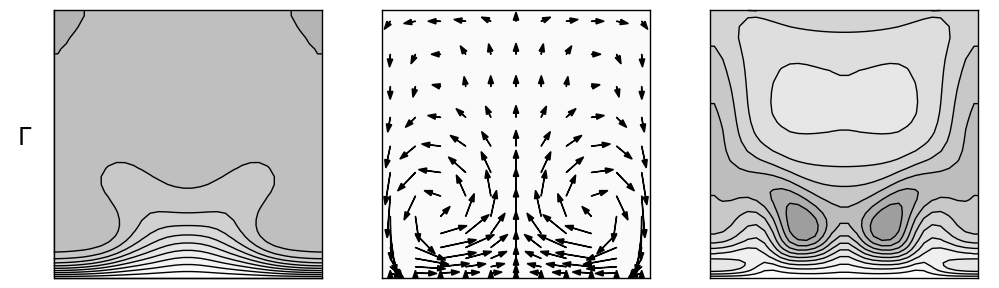
\includegraphics[width=0.9\linewidth]{ductTW-turb1400up-means.png}}
\caption{Поле скорости нескольких бегущих волн: изолинии средней продольной скорости (столбец 1), векторное поле средней поперечно скорости (столбец 2) и линии равного уровня амплитуды колебаний (столбец 3) в сечении $x = 0$. Каждая строка соответствует одному решению. Твердая стенка внизу.} 
\label{ductTW_means_pic}
\end{figure}

Разделим поле скорости бегущих волн $\v_\mathrm{tw}$ на среднюю $\V_\mathrm{tw} = \overline{\v_\mathrm{tw}}^x$ и пульсационную $\v'_\mathrm{tw} = \v_\mathrm{tw} - \V_\mathrm{tw}$ составляющие осреднением по продольной координате $x$. Во всех случаях средняя составляющая движения включает полосы повышенной и пониженной скорости. Распределение средней скорости приведено на рис. \ref{ductTW_means_pic} в первом столбце. В центральной части расчетной области, где медленная жидкость проникает ближе к центру канала (верхней границе расчетной области), расположены полосы пониженной скорости. При больших и меньших значениях $z$ на границах расчетной области расположены полосы повышенной скорости. Существование полос во всех решениях поддерживается слабым движением в нормальной к основному потоку плоскости. Распределение средней поперечной скорости, представленное на рис. \ref{ductTW_means_pic} во втором столбце, соответствует наличию стационарных продольных вихрей, поддерживающих существование полос. Там, где медленная жидкость движется от стенки, находятся полосы пониженной скорости. Там, где жидкость движется ближе к стенке --- полосы повышенной скорости. В решении А средняя поперечная скорость не превышает $0.005U$, в решениях Б и В --- $0.04U$, в решении Г --- $0.08U$. Интенсивность поперечного движения в различных решениях отличается почти в 20 раз. 

\begin{figure}
\center{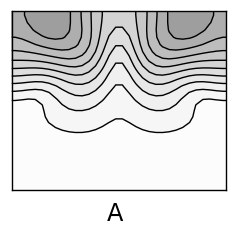
\includegraphics[width=0.25\linewidth]{ductTW-edge2000low-lin.png}
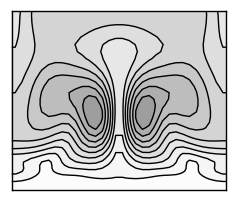
\includegraphics[width=0.25\linewidth]{ductTW-edge2000up-lin.png}
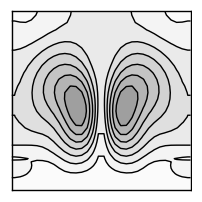
\includegraphics[width=0.22\linewidth]{ductTW-turb1400low-lin.png}
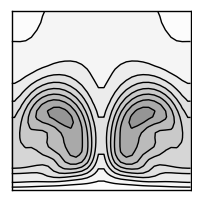
\includegraphics[width=0.22\linewidth]{ductTW-turb1400up-lin.png}}
\caption{Линии равного уровня амплитуды колебаний для собственных решений линейной задачи устойчивости среднего течения нескольких бегущих волн. Твердая стенка внизу.} 
\label{ductTW_lin_pic}
\end{figure}

Колебания во всех решениях оказываются сконцентрированы в областях, где градиент средней продольной скорости имеет наибольшее значение --- между полосами повышенной и пониженно скорости. Амплитуда пульсаций приведена на рис. \ref{ductTW_means_pic} в третьем столбце. В решении А, найденном на сепаратрисе, пульсации достигают максимума в центральной части канала, на наибольшем удалении от стенки. Максимальное значение амплитуды колебаний составляет $0.025U$. В других решениях пульсации достигают максимума ближе к твердой стенке, а максимальная амплитуда колебаний оказывается выше: $0.06U$ для решения Б, $0.083U$ для решения В и $0.15U$ для решения Г. Амплитуда колебаний в решении А отличается от амплитуды колебаний в решении Г почти в 10 раз. 

Мы полагаем, что во всех случаях пульсации образуются в результате линейной неустойчивости полосчатого движения. 
Среднее поле скорости решения А оказывается линейно неустойчивым. Инкремент нарастания наиболее быстро растущего собственного решения равен $\lambda_1 = 0.0001U/H$. Собственная функция наиболее быстрорастущего решения с большой точностью повторяет форму пульсационной составляющей движения и ее фазовую скорость, что позволяет сделать вывод о том, что пульсации в решении возникают в результате линейной неустойчивости среднего течения. Амплитуда колебаний для наиболее быстрорастущей собственной функции приведена на рис. \ref{ductTW_lin_pic}(А), ее фазовая скорость равна $c_1=0.97U$. 

Среднее поле скорости решения Б оказывается устойчивым к малым возмущениям (имеющим $5R$ периодичность вдоль трубы), однако и в этом случае наиболее медленно затухающее собственное решение повторяет форму пульсационной составляющей движения и имеет близкую фазовую скорость. Декремент затухания собственного решения равен $\lambda_1 = -0.0008U/R$, фазовая скорость $c_1 = 0.7U$, амплитуда колебаний для соответствующей собственной функции приведена на рис. \ref{ductTW_lin_pic}(Б). Линейная устойчивость среднего течения не противоречит представлению о том, что механизм передачи энергии в пульсационную составляющую движения является линейным. Градиенты в среднем поле скорости несколько ниже, чем в неосредненном, соответственно, среднее поле скорости более устойчиво, чем неосредненное. 

Среднее поле скорости решения В оказывается линейно неустойчивым и собственная функция, соответствующая наиболее быстрорастущему собственному решению, с большое точностью повторяет форму пульсационной составляющей движения и ее фазовую скорость. Инкремент нарастания наиболее быстрорастущего решения равен $\lambda_1 = 0.0059U/H$, его фазовая скорость $c_1 = 0.79U$, амплитуда колебаний приведена на рис. \ref{ductTW_lin_pic}(В). 

\begin{figure}
\center{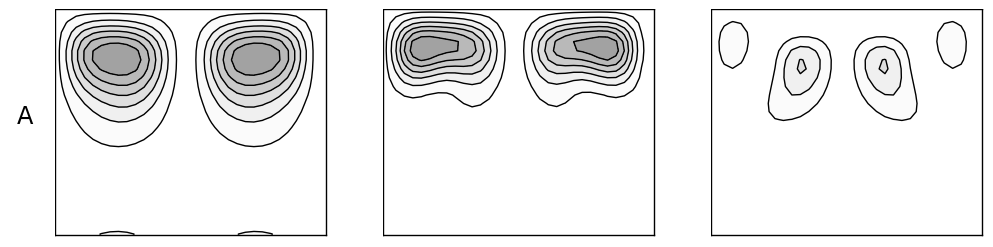
\includegraphics[width=0.9\linewidth]{ductTW-edge2000low-OXgen.png}}
\center{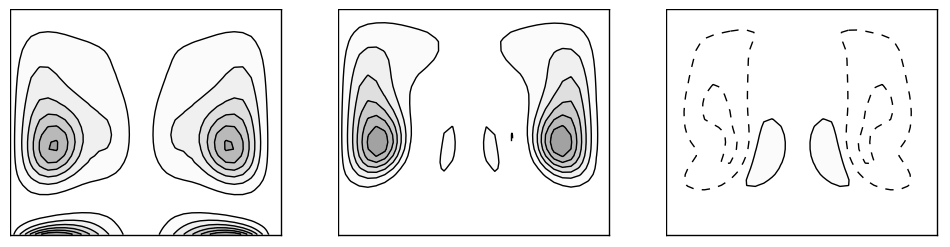
\includegraphics[width=0.9\linewidth]{ductTW-edge2000up-OXgen.png}}
\center{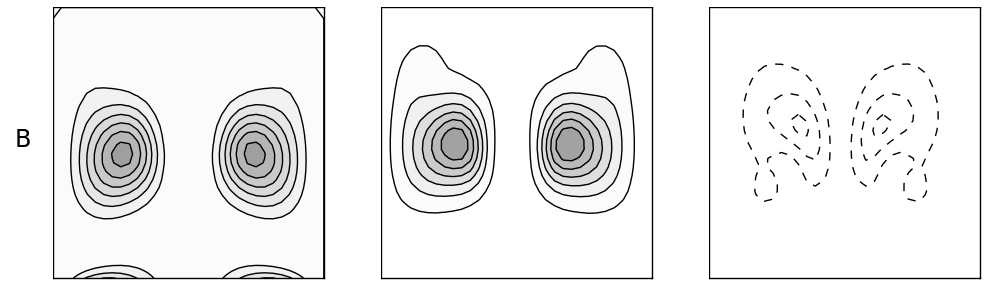
\includegraphics[width=0.9\linewidth]{ductTW-turb1400low-OXgen.png}}
\center{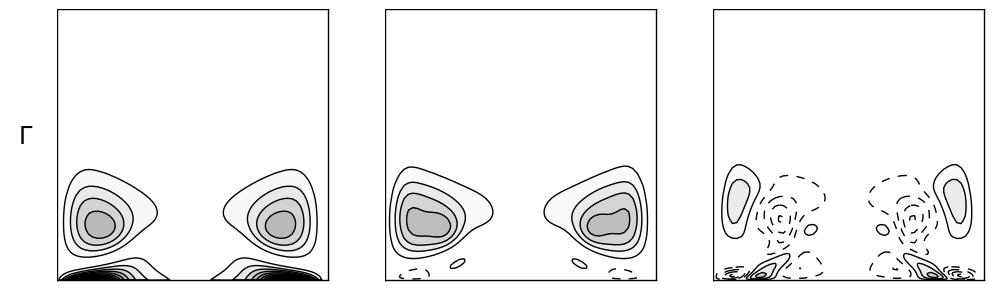
\includegraphics[width=0.9\linewidth]{ductTW-turb1400up-OXgen.png}}
\caption{Механизм образования продольных вихрей: распределение квадрата средней продольной завихренности $\Omega_x^2$ (столбец 1), вклад в образование $\Omega_x^2$ со стороны слагаемых, соответствующих слагаемым \eqref{OXgen_terms} (столбец 2) и сумме других слагаемых в правой части \eqref{OX1_eq} (столбец 3). Каждая строка соответствует одному решению. Сплошные линии --- положительные значения, прерывистые -- отрицательные. Твердая стенка внизу.}
\label{ductTW_OXgen_pic}
\end{figure}

Поле скорости решения Г также оказывается линейно неустойчивым. В этом случае собственная функция, соответствующая наиболее быстрорастущему собственному решению, не так точно повторяет форму пульсационной составляющей движения, но воспроизводит ее основные черты. В частности, собственная функция соответствует синусоидальной неустойчивости (возмущения антисимметричны относительно плоскости $z = Z_\mathrm{max} / 2$, проходящей через полосу пониженной скорости); пульсации оказываются сосредоточены между полосами повышенной и пониженной скорости; близки значения фазовых скоростей. Инкремент нарастания наиболее быстрорастущего собственного решения равен $\lambda_1 = 0.0081U/H$, его фазовая скорость равна $c_1 = 0.7U$, амплитуда колебаний приведена на рис. \ref{ductTW_lin_pic}(Г). Значительные различия в форме пульсационной составляющей движения и собственной функции линейной задачи устойчивости, по-видимому, связаны с существенной ролью нелинейных слагаемых в эволюции пульсационной составляющей движения ввиду их большой амплитуды. 

За образование стационарных продольных вихрей во всех исследованных решениях отвечает выделенный в главе \ref{OXgen_ch} механизм. Продольным вихрям соответствуют области концентрации положительной и отрицательной средней продольной завихренности $\Omega_x$. Для того, чтобы установить механизм образования продольных вихрей, обратимся к уравнению баланса средней продольной завихренности \eqref{OX_eq}. В скалярных переменных в декартовой системе координат это уравнение имеет вид:
\begin{multline}\label{duct_OX1_eq}
\pd{\Omega_x}{t} + V_y \pd{\Omega_x}{y} + V_z \pd{\Omega_x}{z} - \nu\left(\pd{^2\Omega_x}{y^2} + \pd{^2\Omega_x}{z^2}\right)= \\
 - \overline{v'_x \pd{\omega'_x}{x}}^x - \overline{v'_y \pd{\omega'_x}{y}}^x - \overline{v'_z \pd{\omega'_x}{z}}^x
 + \overline{\omega'_x \pd{v'_x}{x}}^x + \overline{\omega'_y \pd{v'_x}{y}}^x + \overline{\omega'_z \pd{v'_x}{z}}^x.
\end{multline}
Здесь $V_y, V_z$ --- нормальная к стенке и трансверсальноая компоненты средней скорости $\V_\mathrm{tw}$, $(v'_x, v'_y, v'_z)$ и $(\omega'_x, \omega'_y, \omega'_z)$ --- компоненты пульсационных составляющих скорости $\v'$ и завихренности $\om' = \rot \v'_\mathrm{tw}$. Второе, третье и четвертое слагаемые в левой части уравнения отвечают за конвекцию $\Omega_x$ в плоскости поперечного сечения и эффект вязкости. Слагаемые в правой части уравнения ответственны за производство средней продольной завихренности, обусловленное наличием пульсаций скорости. Обнаружено, что определяющий вклад в производство средней продольной завихренности вносят только два слагаемых:
\begin{equation}\label{duct_OXgen_terms}
- \overline{v'_x \frac{\d \omega'_x}{\d x}}^x + \overline{ \omega'_x \frac{\d v'_x}{\d x} }^x.
\end{equation}
В силу продольной периодичности оба слагаемых тождественно равны друг другу. Для того, чтобы продемонстрировать роль выделенных слагаемых, обратимся к уравнению баланса квадрата средней продольной завихренности $\Omega_x^2$, полученного умножением \eqref{duct_OX1_eq} на $2\Omega_x$. Положительное значение слагаемых в этом уравнении говорит об их положительном вкладе в производство $\Omega_x$, а отрицательное значение --- об отрицательном вкладе. Значение слагаемых \eqref{duct_OXgen_terms}, умноженных на $2\Omega_x$, приведено на рис. \ref{ductTW_OXgen_pic} во втором столбце, в третьем столбце приведено значение суммы других слагаемых в правой части \eqref{duct_OX1_eq}, также умноженных на $2\Omega_x$. Во всех случаях выделенные слагаемые существенно превосходят другие источниковые слагаемые по величине и определяют форму поля средней продольной завихренности, квадрат которой приведен на том же рисунке в первом столбце. Значение других источниковых членов в решении А дает незначительной положительный вклад в производство $\Omega_x$. В решении В они, напротив, дают незначительный отрицательный вклад. В решениях Б и Г другие слагаемые дают достаточно существенный как положительный, так и отрицательный вклады, но их суммарный эффект также близок к нулю. 

\begin{figure}
\center{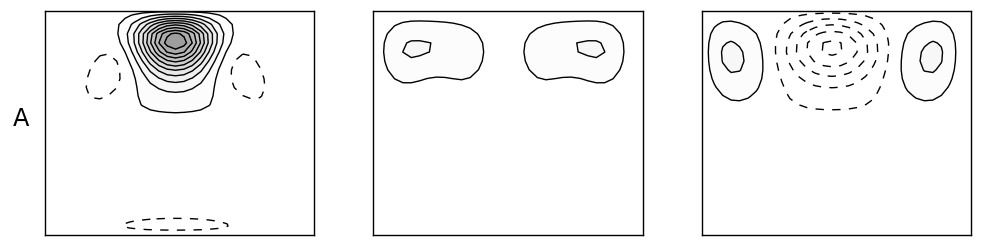
\includegraphics[width=0.9\linewidth]{ductTW-edge2000low-ox1gen.png}}
\center{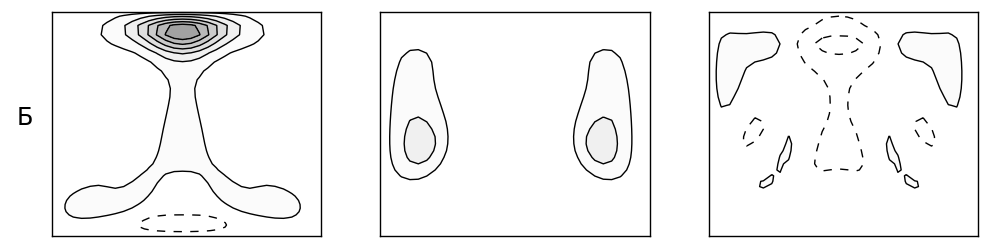
\includegraphics[width=0.9\linewidth]{ductTW-edge2000up-ox1gen.png}}
\center{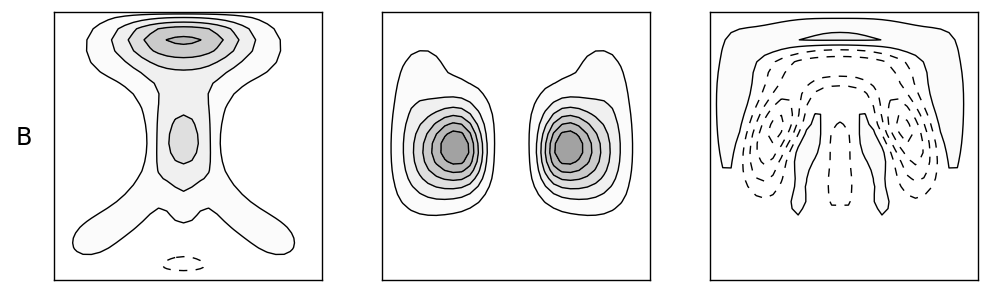
\includegraphics[width=0.9\linewidth]{ductTW-turb1400low-ox1gen.png}}
\center{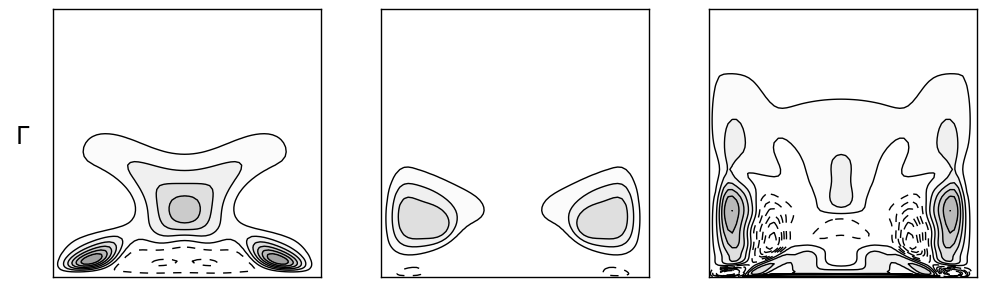
\includegraphics[width=0.9\linewidth]{ductTW-turb1400up-ox1gen.png}}
\caption{Механизм образования пульсаций продольной завихренности: вклад в образование $\overline{\omega'_x\omega'_x}^x$ со стороны слагаемых, соответствующих слагаемым \eqref{ox1gen_add_terms} (столбец 1), слагаемому \eqref{ox1gen_main_terms} (столбец 2) и сумме других слагаемых в правой части \eqref{OX1_eq} (столбец 3). Каждая строка соответствует одному решению. Сплошные линии --- положительные значения, прерывистые -- отрицательные. Твердая стенка внизу. }
\label{ductTW_ox1gen_pic}
\end{figure}

Отличие от нуля слагаемых \eqref{duct_OXgen_terms} говорит о наличии корреляции между пульсациями продольной скорости и пульсациями продольной завихренности. Объяснить наличие такой корреляции позволяет механизм образования пульсаций продольной завихренности. Для того, чтобы установить этот механизм, обратимся к уравнению эволюции пульсационной составляющей продольной завихренности \eqref{ox1_eq}. В скалярных переменных в декартовой системе координат это уравнение имеет вид:
\begin{multline}\label{duct_ox2_eq}
\pd{\omega'_x}{t} + (V_x - c_\mathrm{tw})\pd{\omega'_x}{x} + V_y \pd{\omega_x'}{y} + V_z \pd{\omega'_x}{z} - \nu\nabla^2\omega'_x = \\
- v'_y \pd{\Omega_x}{y} - v'_z \pd{\Omega_x}{z} 
+ \Omega_x \pd{v'_x}{x} + \Omega_y \pd{v'_x}{y} + \Omega_z \pd{v'_x}{z}
+ \omega'_y \pd{V_x}{y} + \omega'_z \pd{V_x}{z} - \\ 
- v'_x \pd{\omega'_x}{x} - v'_y \pd{\omega'_x}{y} - v'_z \pd{\omega'_x}{z} 
+ \omega'_x \pd{v'_x}{x} + \omega'_y \pd{v'_x}{y} + \omega'_z \pd{v'_x}{z} + \\
+ \overline{v'_x \pd{\omega'_x}{x}}^x + \overline{v'_y \pd{\omega'_x}{y}}^x + \overline{v'_z \pd{\omega'_x}{z}}^x
- \overline{\omega'_x \pd{v'_x}{x}}^x - \overline{\omega'_y \pd{v'_x}{y}}^x - \overline{\omega'_z \pd{v'_x}{z}}^x.
\end{multline}
Здесь $V_x$ --- средняя продольная скорость, $\Omega_y, \Omega_z$ --- нормальная к стенке и трансверсальная компоненты средней завихренности $\Om = \rot \V_\mathrm{tw}$. Второе, третье и четвертое слагаемые в правой части уравнения \eqref{duct_ox2_eq} отвечают за конвекцию пульсаций продольной скорости. Уравнение записано в системе отсчета, перемещающейся со скоростью бегущей волны $c_\mathrm{tw}$. Последнее слагаемое в левой части уравнения описывает эффект вязкости. Слагаемые в правой части уравнения описывают различные механизмы образования пульсаций продольной завихренности. В этом уравнении мы выделяем две группы слагаемых, играющих наиболее существенную роль в поддержании $\omega'_x$:
\begin{equation}\label{duct_ox1gen_add_terms}
\pd{\omega'_x}{t} = \omega'_y \pd{V_x}{y} + \Omega_z \pd{v'_x}{z} + 
\end{equation}
\begin{equation}\label{duct_ox1gen_main_terms}
+ \Omega_x \frac {\d v'_x}{\d x} + \dots
\end{equation} 
Слагаемые \eqref{duct_ox1gen_add_terms} отвечают за поворот нормальных к стенке вихрей на фоне нормального к стенке градиента скорости и дают существенный вклад в поддержание пульсаций $\omega'_x$, но производимые этими слагаемыми пульсации $\omega'_x$ не могут участвовать в поддержании продольных вихрей, так как не имеют необходимой для этого согласованности фаз с пульсациями $v'_x$ (подробности в разделе \ref{ox1gen_seq}). Доминирующую роль в поддержании пульсаций $\omega'_x$ в области расположения продольных вихрей играет слагаемое \eqref{duct_ox1gen_main_terms}. Именно это слагаемое обеспечивает необходимую для поддержания продольных вихрей согласованность фаз. 

Для того, чтобы получить представление о роли различных слагаемых уравнения \eqref{duct_ox2_eq} в формирование $\omega'_x$, обратимся к уравнению баланса среднего квадрата пульсаций продольной завихренности $\overline{\omega'_x \omega'_x}^x$, полученного умножением \eqref{duct_ox2_eq} на $2\omega'_x$ с последующим осреднением по $x$. Слагаемые в этом уравнении зависят только от $y$ и $z$, что дает возможность привести их значение на рисунках. Положительное значение источниковых членов в этом уравнении говорит об их положительном вкладе в поддержание $\omega'_x$, а отрицательное значение --- об отрицательном вкладе. На рис. \ref{ductTW_ox1gen_pic} в первом столбце приведено значение слагаемых \eqref{duct_ox1gen_add_terms}, осредненные по $x$ вместе с $2\omega'_x$, во втором столбце приведено значение слагаемого \eqref{duct_ox1gen_main_terms}, осредненного по $x$ вместе с $2\omega'_x$, а в третьем столбце приведено значение суммы других слагаемые из правой части \eqref{duct_ox2_eq}, также осредненных по $x$ вместе с $2\omega'_x$. Хотя слагаемые \eqref{duct_ox1gen_add_terms} дают существенный вклад в производство $\omega'_x$, в области расположения продольных вихрей их влияние незначительно. Зато вклад слагаемого \eqref{duct_ox1gen_main_terms} сосредоточен именно в области расположения продольных вихрей и определяет форму пульсаций $\omega'_x$ в этой области. Другие источниковые члены на месте продольных вихрей дают существенный как положительный, так и отрицательный вклад, но их суммарное влияние близко к нулю. Кроме того, именно слагаемое \eqref{duct_ox1gen_main_terms} дает необходимую для поддержания продольных вихрей согласованность фаз между $\omega'_x$ и $v'_x$. Даже если другие слагаемые из правой части \eqref{duct_ox2_eq} оказывают существенное влияние на форму пульсаций $\omega'_x$, эти изменения формы в значительно меньшей степени влияют на значение слагаемых \eqref{duct_OXgen_terms}, поддерживающих существование продольных вихрей.

Слагаемое \eqref{duct_ox1gen_main_terms} отвечает за растяжение и сжатие существующих в потоке вихревых нитей, обусловленное наличием пульсаций продольной скорости. Это слагаемые стремится произвести пульсации $\omega'_x$, пропорциональные пульсациям $\partial v'_x / \partial x$, причем коэффициентом пропорциональности выступает $\Omega_x$. Соответственно, в области расположения положительного вихря пульсации $\omega'_x$ и $\partial v'_x / \partial x$ положительно пропорциональны, а в области расположения отрицательного --- отрицательно пропорциональны. Именно такое соотношение фаз обеспечивает наибольшую эффективность поддержания продольных вихрей. Подробности в разделе \ref{ox1gen_seq}. 

Таким образом, все основные элементы механизма поддержания колебаний в исследованных бегущих волнах в плоском течении Пуазейля совпадают с выделенными в первой части работы при исследовании модельного порыва. Можно отметить несколько отличий. Во-первых, в случае решения Б среднее течение оказалось линейно устойчивым, но это не противоречит тому, что энергия в пульсационную составляющую движения передается линейным механизмом. То, что механизм передачи энергии действительно линейный, подтверждается тем, что собственная функция, соответствующая наиболее медленно затухающему решению, и в этом случае с высокой точностью повторяет форму и фазовую скорость пульсационной составляющей движения. Во-вторых, в случае решения Г собственная функция, соответствующая наиболее быстрорастущему собственному решению линейной задачи устойчивости среднего течения, не очень точно повторяет форму пульсационной составляющей движения. По-видимому, такая особенность объясняется высокой амплитудой колебаний в этом случае и существенной ролью нелинейных слагаемых в уравнении эволюции пульсационной составляющей движения. Качественное согласие между решением линейной задачи и пульсационной составляющей движения и в этом случае сохраняется. В-третьих, слагаемое \eqref{ox1gen_main_terms} в уравнении \eqref{ox2_eq} оказывается не единственным, оказывающим существенное влияние на форму $\omega'_x$ в области расположения продольных вихрей. Тем не менее, именно это слагаемое порождает пульсации $\omega'_x$, согласованные с $v'_x$ необходимым для поддержания продольны вихрей образом, и именно это слагаемое имеет постоянное значение во всей области существования продольны вихрей. 


\section{Выводы по главе}

В главе представлены результаты исследования нескольких семейств инвариантных решений уравнений Навье-Стокса. Продолжение модельного порыва по параметру позволило получить семейство условно периодических решений с пространственно-локализованной структурой. В геометрии круглой трубы и плоского канала найдено несколько семейств решений, имеющих вид бегущей волны. Найденные решения существенно отличаются друг от друга по форме, интенсивности различных компонент движения, геометрии расчетной области. Тем не менее, все найденные решения воспроизводят общий механизм поддержания колебаний, согласующийся с механизмом поддержания колебаний, выделенном при исследовании модельного порыва, что в некотором смысле говорит об универсальности этого механизма. Некоторые различия в деталях не противоречат уже сложившимся представлениям о нем. То обстоятельство, что выделенный в течении Гагена-Пуазейля механизм поддержания колебаний ответственен также за поддержание колебаний в плоском течении Пуазейля, говорит об отсутствие существенного влияния кривизны стенки на этот механизм. То, что выделенный механизм отвечает за поддержание колебаний в решениях, имеющих вид бегущей волны, говорит об отсутствии существенного влияния не этот механизм пространственно-локализованной структуры решения. Отметим также, что все исследованные решения найдены при схожих условиях симметрии. Существует возможность того, что при других условиях симметрии или в их отсутствии структура течения может качественно измениться.






